% -*- latex -*-


\chapter{Introduction}
\label{chap:Introduction}

The Image Composition Engine for Tiles (\IceT) is an API designed to enable
OpenGL applications to perform Sort-Last parallel rendering on very large
displays.  The displays are assumed to be
\index{tiled~display}\keyterm{tiled displays}, which are displays
comprising an array of display devices that act together to form a single
large display.  The overall resolution of the display may be several times
larger than any viewport that may be rendered by a single machine.  It is
also assumed that several processes in the parallel application are
\index{display~process}\keyterm{display processes}.  That is, their entire
display window makes up part of the display.

The design philosophy behind \IceT is to allow very large sets of polygons
to be displayed on very high resolution displays.  As such, fast frame
rates are sacrificed in lieu of very scalable and very high polygon/second
rendering rates.  That said, there are many features in \IceT that allow an
application to achieve interactive rates.  These include image inflation,
floating viewports, active pixel encoding, and data replication.  Together,
these features make \IceT a versatile parallel rendering application that
provides near optimal parallel rendering under most data size and image
size combinations.  As an example, the ParaView
application\footnote{\href{http://www.paraview.org}{http://www.paraview.org}}
is using \IceT for all of its parallel rendering needs ranging from a
desktop sized image to the world's largest tiled displays and from polygon
counts ranging from 1 to 1 million (and growing).

\IceT is designed to take advantage of
\index{spatial~decomposition}\keyterm{spatial decomposition} of the
geometry being rendered.  That is, it works best if all the geometry on
each process is located in as small a region of space as possible.  When
this is true, each process usually projects geometry on only a small
section of the screen.  This results in less work for the compositing
engine.  This is of particular importance for displays with a large number
of pixels.

\IceT can also be used to perform sort-last parallel rendering to a single
display.  Such \index{single-tile~rendering}\keyterm{single-tile rendering}
is simply a special case of the multi-tile display \IceT was designed for.
Many of the optimizations done by \IceT apply to the single-tile mode.
Using \IceT for this purpose is quite worthwhile.  \IceT's performance
should rival that of other such software image compositors.

The rest of this document describes the use of the
\IceT
API.  There are also separate manual pages for each of the functions
described here.  For more details on
\IceT's
algorithms, see:

\begin{quote}
  Kenneth Moreland, Brian Wylie, and Constantine Pavlakos.  ``Sort-last
  parallel rendering for viewing extremely large data sets on tile
  displays,'' In \emph{Proceedings of IEEE Symposium on Parallel and
    Large-Data Visualization and Graphics}, October 2001, pp. 85--154.
\end{quote}


\section{A Parallel Rendering Primer}
\label{sec:Introduction:Parallel_Rendering_Primer}

\IceT requires you to know very little about parallel rendering and their
algorithms.  However, it is helpful to know the basic idea behind \IceT's
algorithms.  This section gives a brief introduction to how \IceT renders
in parallel.

Parallel rendering algorithms are classified as
\index{sort-first}\keyterm{sort-first},
\index{sort-middle}\keyterm{sort-middle}, or
\index{sort-last}\keyterm{sort-last}.  The key distinguishing feature of
each class is how primitives are distributed amongst processes.  As
demonstrated in Figure~\ref{fig:Introduction:ParallelRenderingClasses},
sort-first and sort-middle algorithms allocate screen space to processes
and send the appropriate geometry to each process every frame whereas
sort-last algorithms render static partitions of geometry in each process
and then composite the resulting images to a single image.\footnote{In the
  interest of brevity and clarity, I am intentionally leaving out details
  that are unimportant to understanding \IceT such as hybrid algorithms and
  differences between sort-first and sort-middle algorithms.}  \IceT is a
sort-last parallel rendering library.

\begin{figure}
  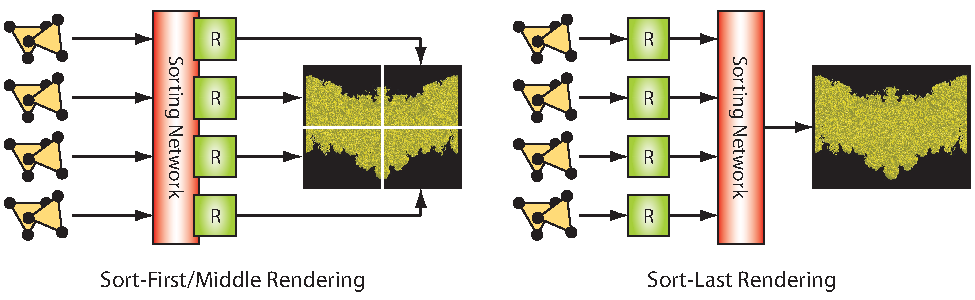
\includegraphics{images/ParallelRenderingClasses}
  \caption[Parallel rendering classes.]{The differences between parallel
    rendering classes.  Sort-first and sort-middle algorithms transfer
    geometric data.  Sort-last algorithms transfer image data.}
  \label{fig:Introduction:ParallelRenderingClasses}
\end{figure}

A convenient feature of sort-last rendering is that an application needs to
change very little about how it renders geometry.  The geometry is rendered
the same in parallel as it is in serial; the only difference is that each
process only renders a subset of the geometry.  The typical operation of a
parallel application using sort-last rendering is to simply render locally
and then composite the images.

When rendering to a tiled display, as \IceT allows you to do, there is an
added level of complexity introduced because the graphics system is often
not capable of rendering an image large enough for the entire display.
Thus, image compositing for a tiled display requires a loop that can
iteratively render images for each tile and composite them.  \IceT handles
this looping and interfaces with the rendering functions of your
application through a callback mechanism.  This will be described in the
following chapters.
